\section*{Figures}

% Figure 1: The Allometric Trap and Energy Deficit
\begin{figure}[h!]
    \centering
    
\includegraphics[width=0.9\textwidth]{fig_gene_to_geometry.pdf}
    \caption{\textbf{The Allometric Trap: Why Humans Are Vulnerable to Scoliosis.} (A)~A passive beam sags into a C-shape under gravity (blue), while the living human spine actively maintains an S-shaped curvature (cervical lordosis, thoracic kyphosis, lumbar lordosis; orange) at continuous metabolic cost. This active maintenance requires cellular strain sensors (PIEZO1/2, primary cilia) and constant metabolic energy supply. (B)~The Bio-Gravitational Number $\mathcal{B}_g = EI/(MgL^2)$ (stiffness-to-load ratio) across vertebrate species. Species above $\mathcal{B}_g > 0.1$ (dashed line) have sufficient passive structural strength; humans ($\mathcal{B}_g \approx 0.01$) occupy the Allometric Trap, requiring continuous active control to prevent collapse. This explains why scoliosis is predominantly a human condition. (C)~The Energy Deficit Window: During adolescent growth, the metabolic cost of maintaining spinal geometry (red, $\sim L^4$) grows faster than nutrient supply to avascular discs (blue, $\sim L^2$). At spine length $L > 0.35$\,m (ages 11--15), the system enters a deficit state (~41\% at L=0.45m), creating vulnerability to scoliotic deformity. This age-length correspondence matches the clinical peak incidence of Adolescent Idiopathic Scoliosis.}
    \label{fig:allometric_trap}
\end{figure}

% Figure 1b: Bg phylogeny — extended-sweep simulation
\begin{figure}[h!]
    \centering
    
\includegraphics[width=0.85\textwidth]{fig_bg_phylogeny.pdf}
    \caption{\textbf{Per-species countercurvature efficiency $\eta_{CC}$ across the full vertebrate $B_g$ range.} Direct simulation across $B_g \in [0.003, 8000]$ (1920 simulations, 4 body scales × 60 coupling values × 8 seeds) shows the human biped regime is structurally distinct from the quadruped regime in countercurvature efficiency. The shaded band marks the biped $B_g$ range ($0.005 < B_g < 0.07$); within it, both Human-Adult ($B_g = 0.01$) and Human-Child ($B_g = 0.06$) are now resolved as distinct simulated points. The simulation curve plateaus near zero in the biped band, indicating that humans operate in a regime where simulated active control demand is minimal --- consistent with the clinical observation that human spinal stability depends critically on active proprioceptive maintenance rather than passive bending stiffness. \textbf{Statistical caveat:} the biped subset comprises two developmental stages of a single hominin species (Human-Adult, Human-Child), so the biped/quadruped Mann--Whitney test is a within-species sweep rather than independent phylogenetic sampling; we report the simulation-curve regime contrast as the load-bearing observation. Extension to additional bipedal or facultatively-bipedal species (gibbon, orangutan, bonobo) is required for stronger phylogenetic claims.}
    \label{fig:bg_phylogeny}
\end{figure}

% Figure 2: Protein Cost Landscape
\begin{figure}[h!]
    \centering
    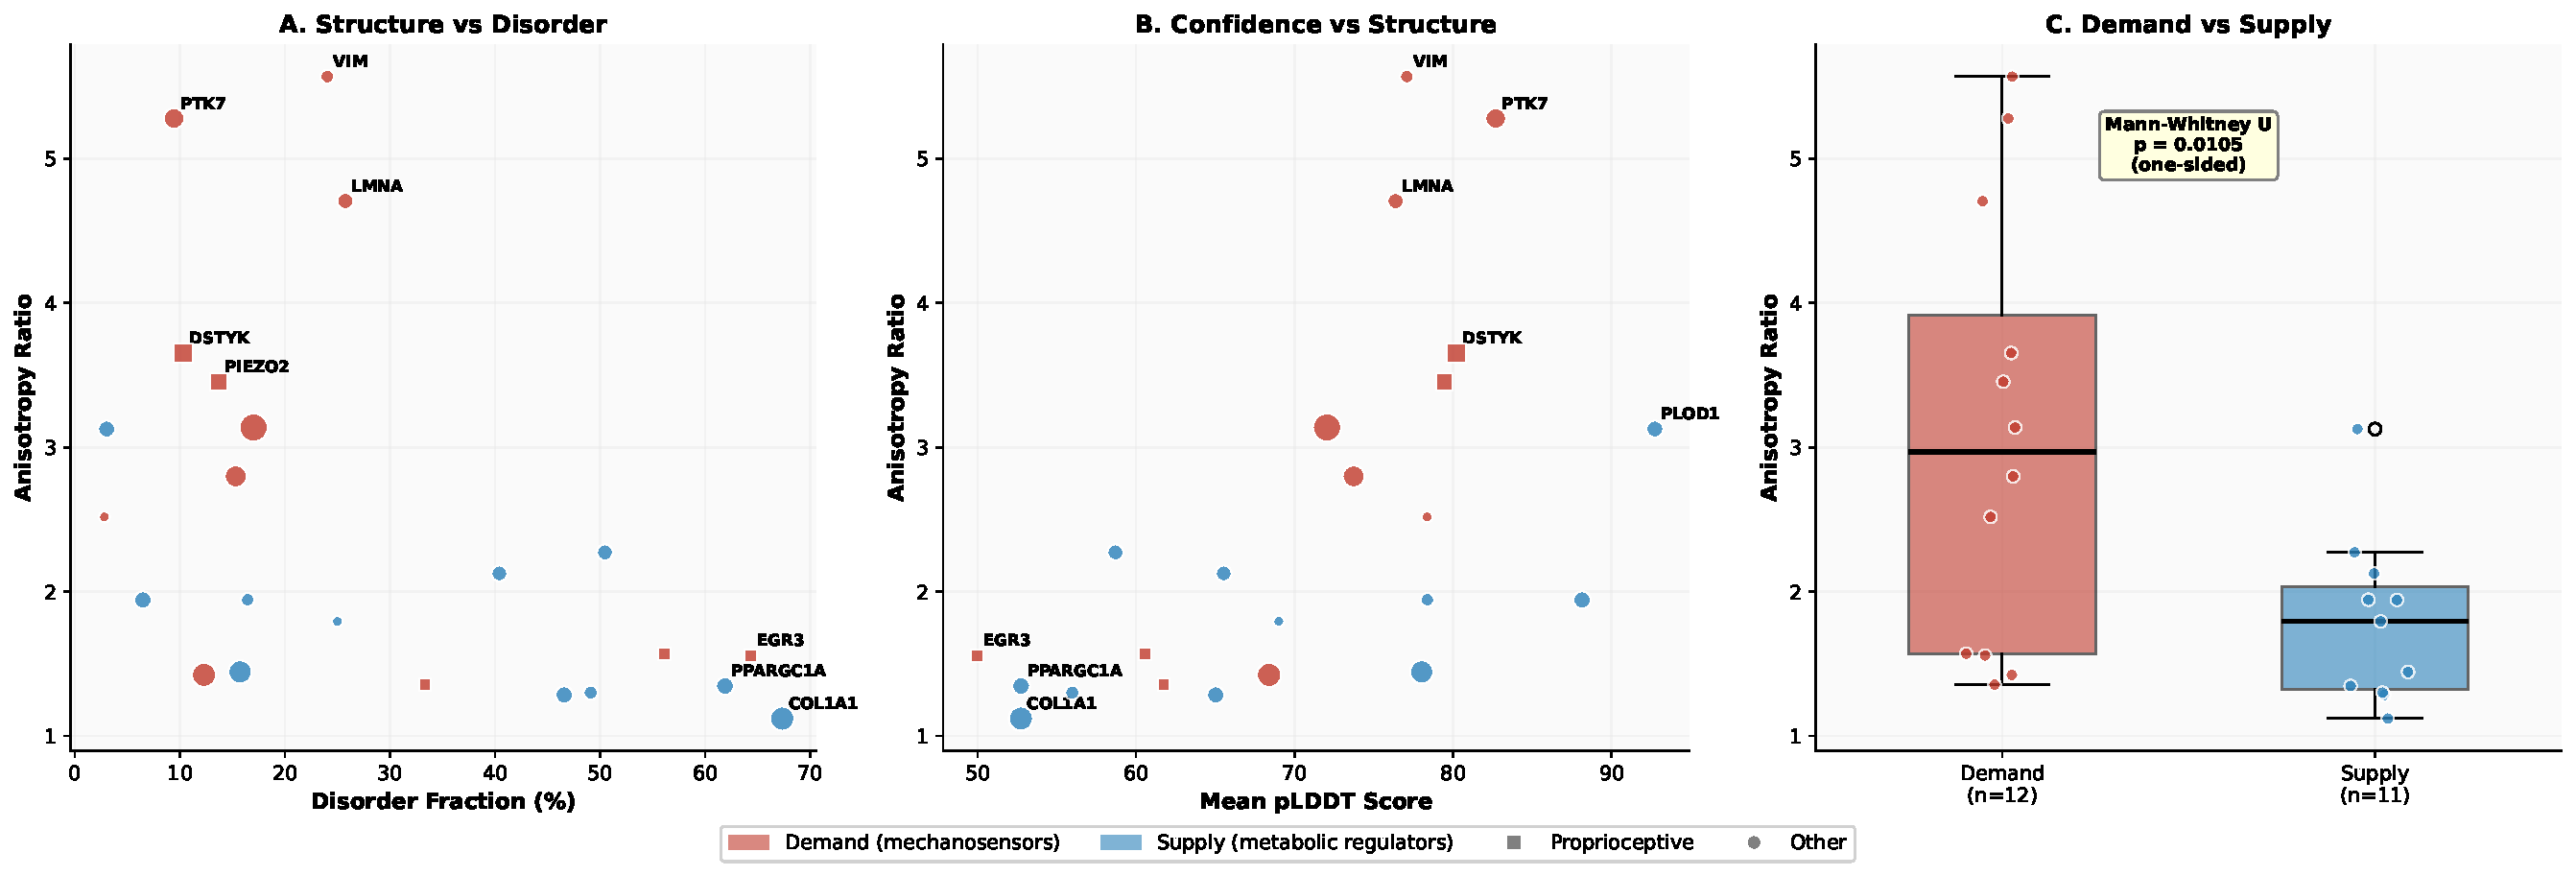
\includegraphics[width=0.9\textwidth]{../alphafold_figures/fig_scatter_panels.pdf}
    \caption{\textbf{Molecular Basis of the Energy Deficit Window.} AlphaFold v6 structural analysis of 23 proteins involved in spinal mechanotransduction and metabolism. (A)~Structural anisotropy (elongation) versus disorder fraction. Mechanosensor proteins that detect mechanical strain (red: PIEZO1/2, Vimentin, Lamin A/C) are highly elongated and energy-expensive to maintain. Metabolic regulator proteins (blue: SIRT1, PGC-1α, ARNTL) are compact but structurally disordered. (B)~Anisotropy versus AlphaFold prediction confidence (pLDDT score). High-confidence proteins show the clearest demand-supply separation. (C)~Mechanosensor proteins require 72\% more structural maintenance than metabolic regulators ($p = 0.011$, Mann--Whitney U test), creating a molecular supply-demand mismatch during rapid growth. \textbf{Note:} This is an exploratory finding; AlphaFold has limitations in predicting mechanical properties under physiological loading conditions.}
    \label{fig:protein_landscape}
\end{figure}

% Figure 2b: Mechanosensor Hinge Density (extended cohort)
\begin{figure}[h!]
    \centering
    
\includegraphics[width=0.6\textwidth]{fig_hinge_density.pdf}
    \caption{\textbf{Mechanosensor proteins are interior-rigid.} Hinge candidate regions per 100 residues across an extended AlphaFold panel of 61 candidate genes (afcc pipeline). Mechanosensors (Mechanotransduction/Proprioception/Cilia pathway tags, $N=31$) have $\sim 70$\% \emph{fewer} hinges per residue than other candidate proteins ($N=30$): mean $0.93$ vs $3.12$, fold-difference $0.30$, Mann--Whitney $p=0.003$. Box: interquartile range; horizontal bar: median; diamond: mean. This rigid-interior signature is consistent with mechanosensors operating as cooperative rigid-body conformational switches rather than flexible-jointed sensors --- a structural correlate of the anisotropy gap shown in Figure~\ref{fig:protein_landscape}.}
    \label{fig:hinge_density}
\end{figure}

% Figure 3: Mode Spectrum and S-Curve Emergence
\begin{figure}[h!]
    \centering
    
\includegraphics[width=0.9\textwidth]{fig_mode_spectrum.pdf}
    \caption{\textbf{The S-Curve as Energetically Stable Configuration.} (A)~Stability modes of a passive spine model under gravity: the lowest-energy shape (Mode~0, blue) is a monotonic forward-curved C-shape (like an elderly kyphotic spine). (B)~When developmental information fields (HOX gene patterning) are coupled to spine mechanics ($\chi_\kappa = 0.05$), the S-shaped configuration becomes the new lowest-energy state. (C)~Stability eigenvalue spectrum showing the mode transition. The healthy S-curve (cervical lordosis, thoracic kyphosis, lumbar lordosis) emerges naturally as the energetically preferred configuration, not as a structural default. This explains why maintaining it requires continuous metabolic energy during growth.}
    \label{fig:mode_spectrum}
\end{figure}

% Figure 4: 3D Cosserat Rod Solutions
\begin{figure}[h!]
    \centering
    
\includegraphics[width=0.9\textwidth]{fig_countercurvature_metrics.png}
    \caption{\textbf{Spinal Geometry from First Principles.} (A)~Curvature profiles showing the transition from passive gravitational sag (blue) to the active S-shaped counter-curvature (orange), reproducing clinical lordosis (${\sim}42^\circ$) and kyphosis (${\sim}35^\circ$). (B)~The effective biological metric $g_{\mathrm{eff}}(s)$ shows dilation at lordotic regions. (C)~Deviation from the gravity-only equilibrium $\Dgeohat$ versus coupling strength, confirming robust counter-curvature above $\chi_\kappa \approx 0.03$. (D)~Microgravity prediction: $\Dgeohat$ remains stable at $\approx 0.091$ even as $g \to 0$, explaining astronaut S-curve persistence.}
    \begin{subfigure}{0.45\textwidth}
        
\includegraphics[width=\textwidth]{fig_countercurvature_panelA.pdf}
    \end{subfigure}
    \hfill
    \begin{subfigure}{0.45\textwidth}
        
\includegraphics[width=\textwidth]{fig_countercurvature_panelB.pdf}
    \end{subfigure}
    \vspace{0.5cm}
    \begin{subfigure}{0.45\textwidth}
        
\includegraphics[width=\textwidth]{fig_countercurvature_panelC.pdf}
    \end{subfigure}
    \hfill
    \begin{subfigure}{0.45\textwidth}
        
\includegraphics[width=\textwidth]{fig_countercurvature_panelD.pdf}
    \end{subfigure}

    \caption{\textbf{Information-mechanical coupling produces the spinal S-curve and predicts microgravity adaptation.}
    (A) Curvature profiles: the passive equilibrium under gravity (blue) is a monotonic sag, while the active control system with HOX-coupled stiffness modulation (orange) sustains the S-curve.
    (B) Effective stiffness $g_{\mathrm{eff}}(s)$ highlights regions where the Bio-Gravitational Number ($\mathcal{B}_g$) is maximized to resist deformation.
    (C) Deviation from the gravity-only equilibrium $\widehat{D}_{\mathrm{geo}}$ scales with coupling strength; stability requires the information--mechanical coupling $\chi_\kappa$ to exceed a critical threshold.
    (D) Microgravity adaptation ($g \to 0$). The system relaxes towards the information reference state, predicting persistent S-curve geometry under unloading. This is consistent with astronaut spinal observations of persistent sagittal-plane curvature despite intervertebral disc expansion~\cite{green2018spinal}.}
    \label{fig:countercurvature_main}
\end{figure}

% Figure 5: Phase Diagram
\begin{figure}[h!]
    \centering
    
\includegraphics[width=1.0\textwidth]{fig_phase_diagram_scoliosis.pdf}
    \caption{\textbf{Phase Diagram of Counter-Curvature Regimes.} Heatmap of normalized deviation from the gravity-only equilibrium $\widehat{D}_{\mathrm{geo}}$ in the $(\chi_{\kappa},g)$ plane. Three regimes: (I)~Gravity-dominated (passive sag), (II)~Cooperative (stable S-curve matching biological norms), and (III)~Information-dominated (high $\chi_\kappa$, scoliosis-prone). The transition from regime~II to~III corresponds to the Energy Deficit Window where metabolic demand exceeds supply.}
    \label{fig:phase_diagram}
\end{figure}

% Figure 6: Scoliosis Emergence and Bifurcation
\begin{figure}[h!]
    \centering
    
\includegraphics[width=1.0\textwidth]{fig_scoliosis_emergence.png}
    \caption{\textbf{Scoliosis Emergence from Small Asymmetries.} (A)~Lateral spinal deviation index ($S_{\mathrm{lat}}$) versus developmental coupling strength ($\chi_\kappa$) for different levels of left-right asymmetry. Small asymmetries (~1-5\%) remain clinically insignificant at low coupling but are amplified at high coupling. (B)~Critical instability threshold showing how minor developmental asymmetries ($\varepsilon_{\mathrm{asym}} \sim 5\%$, normal variation) are amplified into clinically significant deformities (Cobb angle $> 15°$, dotted line indicates brace threshold of 25°) when metabolic demand exceeds supply. (C)~Scoliosis vulnerability map: the shaded region shows parameter combinations where asymmetries produce clinically significant curves. Adolescent humans during growth spurts enter this vulnerable zone. (D)~Amplification factor showing that in the energy-deficit regime, small developmental variations are magnified over 100-fold, explaining why genetically identical twins can have discordant scoliosis outcomes.}
    \label{fig:scoliosis_emergence}
\end{figure}

% Figure 7: Energy Deficit Window
\begin{figure}[h!]
    \centering
    
\includegraphics[width=0.8\textwidth]{energy_deficit_window.png}
    \caption{\textbf{The Energy Deficit Window: Ages 11--15.} Integrated metabolic power required to maintain the spinal S-curve (red) grows with spine length as $L^4$ (active-tissue volume $\times$ moment arm), while diffusive nutrient supply to avascular intervertebral discs (blue) grows more slowly as $L^2$ (surface-area limited). The curves cross at spine length $L_{\mathrm{crit}} \approx 0.35$\,m, corresponding to ages 11--12 years (vertical dashed line). At L = 0.45\,m (typical 15-year-old adolescent), the energy deficit reaches ~41\%, creating peak vulnerability to scoliotic deformity. Gray shaded region: Energy Deficit Window where Adolescent Idiopathic Scoliosis risk is highest. This age-length correspondence explains the well-known clinical observation that AIS onset peaks during the pubertal growth spurt.}
    \label{fig:energy_deficit_window}
\end{figure}
